\documentclass[11pt]{beamer}
\usetheme{Boadilla}
\usepackage[utf8]{inputenc}
\usepackage{amsmath}
\usepackage{amsfonts}
\usepackage{amssymb}
\usepackage{booktabs}
\usepackage{svg}
\def\xcolorversion{2.00}
\def\xkeyvalversion{1.8}
\usepackage{pgf}
\usepackage{tikz}
\usetikzlibrary{arrows,shapes,snakes,automata,backgrounds,petri}

\usepackage{mathtools}
\newcommand\givenbase[1][]{\:#1\lvert\:}
\let\given\givenbase
\newcommand\sgiven{\givenbase[\delimsize]}
\DeclarePairedDelimiterX\Basics[1](){\let\given\sgiven #1}
\newcommand\Average{E\Basics}

%\author{Maximilian Bachl}
\title{Congestion Control}
%\setbeamercovered{transparent} 
%\setbeamertemplate{navigation symbols}{} 
%\logo{} 
%\institute{} 
%\date{} 
%\subject{} 
\begin{document}

\begin{frame}
\titlepage
\end{frame}

%\begin{frame}
%\tableofcontents
%\end{frame}

\begin{frame}{Congestion Control}
\begin{itemize}
\item Why Congestion Control? Before congestion control was invented: Everyone sent as much as they pleased $\rightarrow$ \textit{Congestion Collapse}.
\item Goal: Estimate available bandwidth. Don't send too much, don't send too little.
\item Method: Keep a \textit{Congestion Window}
\item E.g. Congestion Window of 5 means that we can have up to 5 packets somewhere in the network.
\end{itemize}
\end{frame}

\begin{frame}{How does Congestion Control work nowadays?}
Simplified:
\begin{itemize}
\item Congestion Window 1 in the beginning of a flow.
\item Upon receiving an acknowledgement (ACK) for a previously sent packet, increase the Congestion Window (cwnd): $$\text{cwnd} = \frac{1}{\text{cwnd}}$$
\item Recently also a bit more sophisticated $\rightarrow$ \textit{CUBIC} etc. 
\item When there is packet loss then we sent too much (buffer of a router on the way overflew) $\rightarrow$ congestion $\rightarrow$ decrease Congestion Window
\item The most common thing to do is $$\text{cwnd} = \frac{\text{cwnd}}{2}$$
\end{itemize}
\end{frame}

\begin{frame}{Problems}
\begin{itemize}
\item Only decrease window on loss $\rightarrow$ That's too late! Decrease before when buffers of routers fill up and latency increases!
\item On wireless connections stochastic packet loss is common $\rightarrow$ TCP thinks it's congestion.
\end{itemize}
\end{frame}

\begin{frame}{Potential Solution}
\begin{itemize}
\item Let's build some machine learning thing!
\item Solutions already exist $\rightarrow$ \textit{TCP ex Machina} by Winstein and Balakrishnan (2013).
\item They simulate networks and learn an optimum congestion control more or less by using a brute force algorithm.
\item Example: Use networks with 1 to 5 senders, RTT from 10 to 100\,ms. Use one set of congestion control rules for 1000 simulations. Then change some parameters and check if it improved (actually they do it in a smarter way)
\item Problem: Training has to be done offline. But it would be nice to have a Congestion Control that learns in real time, online!
\end{itemize}
\end{frame}

\begin{frame}{Other Potential Solution}
\begin{itemize}
\item \textit{PCC: Re-architecting Congestion Control for Consistent High Performance (PCC)} by Dong et al.~(2013).
\item Sender uses rate $r_1$ for some time and then $b_2$ for some time. 
\item Which rate was better? 
\item Use better rate and start experimenting again 
\item Problem: cannot react quickly as it has to wait for a whole measurement period until it changes its action. 
\end{itemize}
\end{frame}

\begin{frame}{Reinforcement Learning}
\centering
\includesvg{figures/Reinforcement_learning_diagram}
\end{frame}

\begin{frame}{Problems with RL}
\begin{itemize}
\item An action is increasing the Congestion Window
\item We can calculate the reward after receiving all ACKs
\item That takes at least one Round Trip Time
\item In the mean time other packets could have arrived
\item Example: We increase the cwnd by 2 packets. So we can send two packets. To evaluate if this action was good we have to get the ACKs of these two packets, which happens after one RTT!
In the meantime another ACK could have arrived. What do we do? Not defined with RL...
\end{itemize}
\end{frame}

\begin{frame}{Partial Actions}
\centering
\includesvg{figures/Reinforcement_learning_diagram_PAL}
\end{frame}

\begin{frame}{Partial Actions: Example}
\begin{itemize}
\item Example: the window is 1.9
\item Increase the window by $0.3$ (action)
\item Send two packets (partial actions).  
\item Receive the ACK for the first packet (feedback). Update the state and perform a new action.
\item Receive the second ACK. Again, we update the state and perform an action. However, because we got all partial rewards of the previous action, we can calculate the reward and update our agent.
\end{itemize}
\textbf{Key point}: We can update the state without receiving the full reward yet.
\end{frame}

%\begin{frame}{Asynchronous Actor Critic}
%\begin{itemize}
%\item A Deep Learning framework for reinforcement learning. Used for learning how to play video games.
%\item Maximize long term reward: \begin{align*}
%R_t = \left(\left(\sum_{i=0}^{k-1} \gamma^ir_{t+i}\right) + \gamma^k V(s_{t+k}; \theta_\text{v})\right),
%\end{align*}
%\item The \textbf{Critic} tries to estimate how much (long-term) reward one can expect considering the current state.
%\end{itemize}
%\end{frame}

\begin{frame}{Asynchronous Actor Critic}
\begin{itemize}
\item A Deep Learning framework for reinforcement learning. Used for learning how to play video games.
\item Maximize expected long term reward: \begin{align*}
R_t = \gamma r_t + (1-\gamma) R_{t+1}
\end{align*}
\item The \textbf{Critic} tries to estimate how much (long-term) reward one can expect considering the current state.
\end{itemize}
\end{frame}

\makeatletter
\begin{frame}{Exponential decay with $\gamma = 0.01$}
    \global\beamer@shrinktrue
    \gdef\beamer@shrinkframebox{
        \setbox\beamer@framebox=\vbox to\beamer@frametextheight{
            \centering
            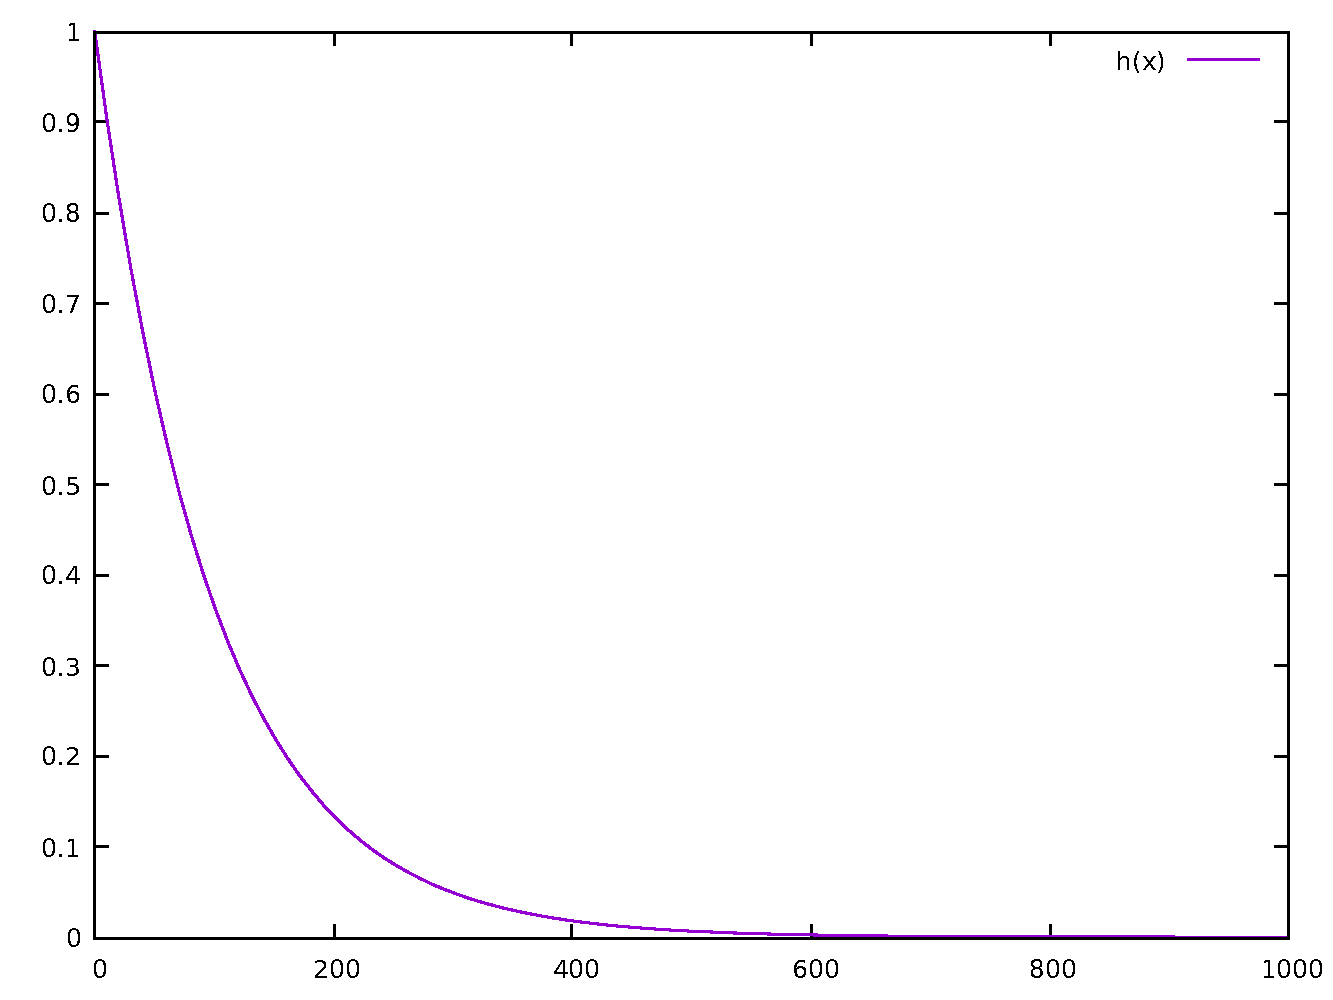
\includegraphics[height=\beamer@frametextheight]{figures/exponential}
        }
    }
\end{frame}
\makeatother

\begin{frame}{Asynchronous Actor Critic -- How to choose $\gamma$}
\begin{itemize}
\item In literature people just set $\gamma = 0.01$. 
\item Problem: The larger the congestion window the more often we'll receive new packets!
\item $\frac{2}{k+1}$ is equivalent to a moving average considering the next $k$ elements.
\item Choose $\frac{2}{w_t+2}$ where $w_t$ is the congestion window at time step $t$.
\end{itemize}
\end{frame}

\begin{frame}{Asynchronous Actor Critic -- Actor}
\begin{itemize}
\item Wants to performs an action that are better than what the Critic would expect.
\item It outputs two things:
\begin{itemize}
\item What it thinks is the best action (e.g. increase the window by $0.3$)
\item A standard deviation to experiment a little bit (e.g. $0.45$)
\end{itemize}
\item So we get a normal distribution from which we sample.
\item Thanks to the standard deviation we experiment and don't get stuck with suboptimal actions. 
\end{itemize}
\end{frame}

\begin{frame}{Neural Network}

\newcommand{\nodedistance}{1.2}
\newcommand{\neuralnetworkwidth}{32}

\pgfmathsetmacro{\shortside}{sqrt((\nodedistance * \nodedistance ) /2)}
\pgfmathsetmacro{\solutionx}{ \shortside }
\pgfmathsetmacro{\solutiony}{ - (3 * \shortside + 3 * \nodedistance ) }

\pgfmathsetmacro{\solutiondurationx}{ \shortside }
\pgfmathsetmacro{\solutiondurationy}{ - (3 * \shortside + 1 * \nodedistance ) }

\centering
\begin{tikzpicture}[every label/.append style={font=\tiny}, node distance=\nodedistance cm, >=stealth',bend angle=45,auto]

  \tikzstyle{place}=[circle,thick,draw=blue!75,fill=blue!20,minimum size=6mm]
  \tikzstyle{input place}=[circle,thick,draw=olive!75,fill=olive!20,minimum size=6mm]
  \tikzstyle{output place}=[circle,thick,draw=magenta!75,fill=magenta!20,minimum size=6mm]
   \tikzstyle{lstm place}=[circle,thick,draw=red!75,fill=red!20,minimum size=6mm]
   \tikzstyle{softplus place}=[circle,thick,draw=green!75,fill=green!20,minimum size=6mm]

  \tikzstyle{transition}=[rectangle,thick,draw=black!75,
  			  fill=black!20,minimum size=4mm]

%  \tikzstyle{every label}=[blue!75]

  \begin{scope}
    \node [input place] (s1) [label={[align=center]left: State (8)}] {};
    \node [place] (s2) [above right of=s1, label={[align=center]above: Linear}] {};
    
  \path[->] (s1) edge node {} (s2);
    
    \node [lstm place] (s3) [right of=s2, label={[align=center]below: GRU (32)}] {};

  \path[->] (s2) edge node {} (s3); 
  \path[->] (s3) edge [loop above] node {} (s3);   
   
    \node [lstm place] (s4) [right of=s3, label={[align=center]below: GRU (32)}] {};    
    
  \path[->] (s3) edge node {} (s4);
  \path[->] (s4) edge [loop above] node {} (s4);
    
    \node [place] (s7) [right of=s4, label={[align=center]below:{ Linear}}] {};
    
  \path[->] (s4) edge node {} (s7);
    
    \node [output place] (s8) [right of=s7, label={[align=center]below: $\sigma$~(1)}] {};    

  \path[->] (s7) edge node {} (s8);

    \node [place] (s5) [above of=s7, label={[align=center]above: Linear}] {};
    
  \path[->] (s4) edge node {} (s5);

    \node [output place] (s6) [right of=s5, label={[align=center]above: $\mu$ (1)}] {};    
    
  \path[->] (s5) edge node {} (s6);    
    
    \node [place] (s10) [below right of=s1, label={[align=center]below: Linear}] {};
    
  \path[->] (s1) edge node {} (s10);

    
    \node [lstm place] (s11) [right of=s10, label={[align=center]above: GRU (32)}] {};
    
  \path[->] (s10) edge node {} (s11);
  \path[->] (s11) edge [loop below] node {} (s11);

    \node [lstm place] (s12) [right of=s11, label={[align=center]above: GRU (32)}] {};
    
  \path[->] (s11) edge node {} (s12);
  \path[->] (s12) edge [loop below] node {} (s12);
    
    \node [place] (s13) [right of=s12, label={[align=center]above: Linear}] {};
    
  \path[->] (s12) edge node {} (s13);

    \node [output place] (s17) [right of=s13, label={[align=center]above: $V_\text{received}$ (1)}] {};
    
  \path[->] (s13) edge node {} (s17);
%    
%    \node [place] (s15) [below of=s13, label={[align=center]above: Linear}] {};
%    
%  \path[->] (s12) edge node {} (s15);
%
%    \node [output place] (s19) [right of=s15, label={[align=center]above: $V_\text{delay}$ (1)}] {};  
    
%  \path[->] (s15) edge node {} (s19);    
    
    \node [place] (s16) [below of=s13, label={[align=center]below: Linear}] {};
    
  \path[->] (s12) edge node {} (s16);    
    
    \node [output place] (s20) [right of=s16, label={[align=center]below: $V_\text{sent}$ (1)}] {};    

  \path[->] (s16) edge node {} (s20);    
    

    \node [place] (s40) at (\solutiondurationx cm,\solutiondurationy cm) [label={[align=center]below: Linear}] {};

  \path[->] (s1) edge node {} (s40);   

    \node [lstm place] (s41) [right of=s40, label={[align=center]above: GRU (32)}] {};
    
  \path[->] (s40) edge node {} (s41);
  \path[->] (s41) edge [loop below] node {} (s41);

    \node [lstm place] (s42) [right of=s41, label={[align=center]above: GRU (32)}] {};
    
  \path[->] (s41) edge node {} (s42);
  \path[->] (s42) edge [loop below] node {} (s42);
       
    \node [place] (s43) [right of=s42, label={[align=center]above: Linear}] {};
    
  \path[->] (s42) edge node {} (s43);
    
    \node [output place] (s44) [right of=s43, label={[align=center]above: $V_\text{duration}$ (1)}] {};   
    
  \path[->] (s43) edge node {} (s44); 
  
%    \node [place] (s17) [below of=s14, label={[align=center]above: Linear}] {};
%    
%  \path[->] (s12) edge node {} (s17);
%    
%    \node [output place] (s22) [right of=s17, label={[align=center]above: $V_\text{byte}$ (1)}] {};   
%    
%  \path[->] (s17) edge node {} (s22);   

%    \node [place] (s30) at (\solutionx cm,\solutiony cm) [label={[align=center]below: Linear}] {};
%
%  \path[->] (s1) edge node {} (s30);   
%
%    \node [lstm place] (s31) [right of=s30, label={[align=center]above: GRU (\neuralnetworkwidth)}] {};
%    
%  \path[->] (s30) edge node {} (s31);
%  \path[->] (s31) edge [loop below] node {} (s31);
%
%    \node [lstm place] (s32) [right of=s31, label={[align=center]above: GRU (\neuralnetworkwidth)}] {};
%    
%  \path[->] (s31) edge node {} (s32);
%  \path[->] (s32) edge [loop below] node {} (s32);
%    
%    \node [place] (s33) [right of=s32, label={[align=center]above: Linear}] {};
%    
%  \path[->] (s32) edge node {} (s33);
%
%    \node [output place] (s34) [right of=s33, label={[align=center]above: $V_\text{byte}$ (1)}] {};
%    
%  \path[->] (s33) edge node {} (s34);

  \end{scope}

\end{tikzpicture}

\end{frame}

\makeatletter
\begin{frame}{Softplus function}
    \global\beamer@shrinktrue
    \gdef\beamer@shrinkframebox{
        \setbox\beamer@framebox=\vbox to\beamer@frametextheight{
            \centering
            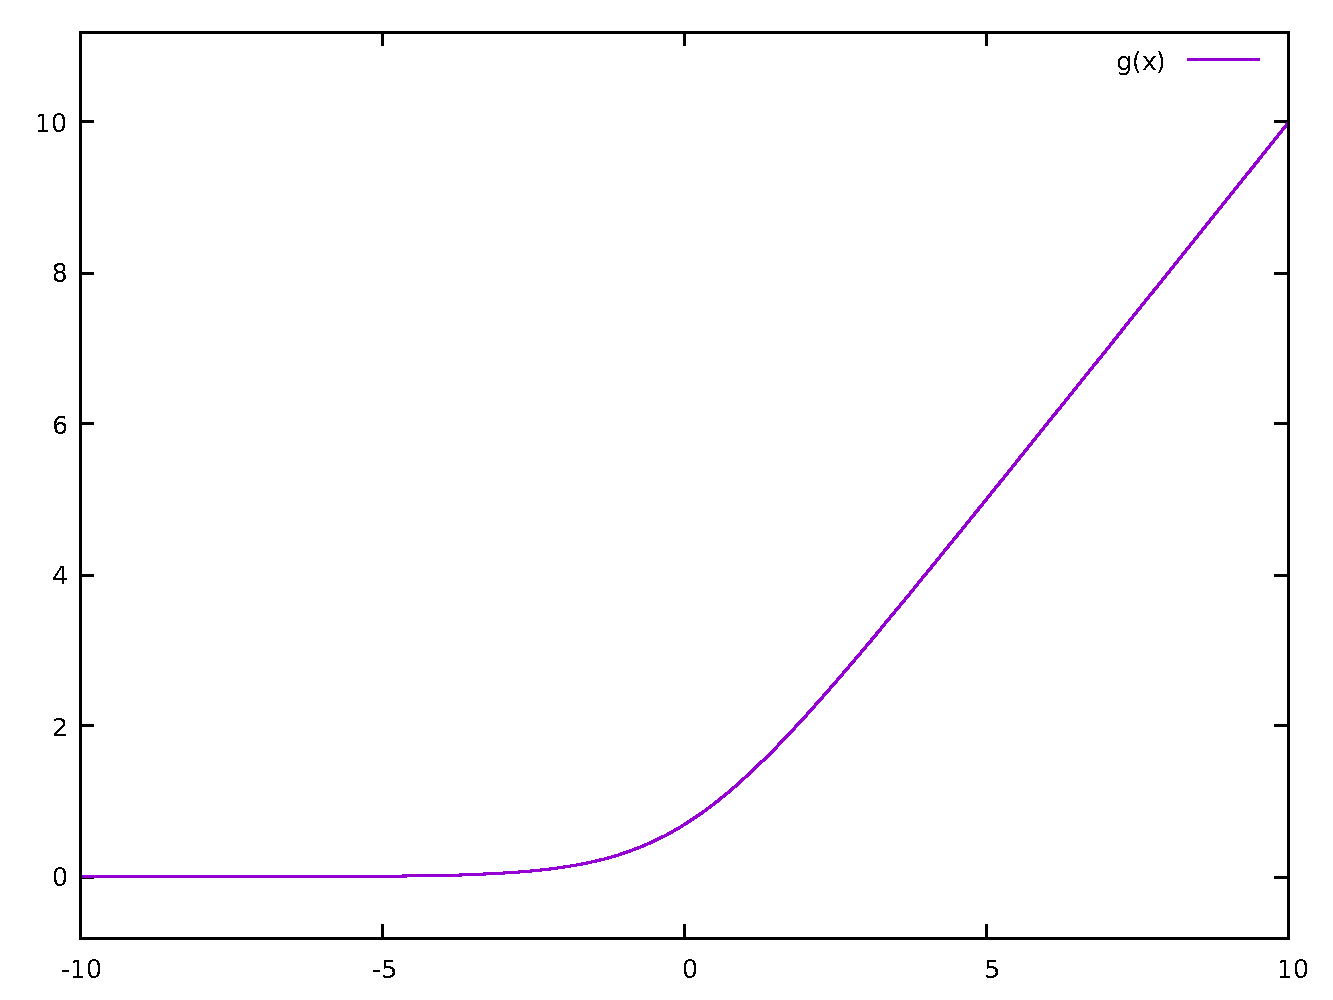
\includegraphics[height=\beamer@frametextheight]{figures/softplus}
        }
    }
\end{frame}
\makeatother

\begin{frame}{Utility function}
\begin{align*}
U_t = \text{throughput} \cdot \text{Sigmoid}_\alpha\left(\text{loss rate} - 0.05 \right) - \text{sending rate}\cdot\text{loss rate}
\end{align*}
\end{frame}

\begin{frame}{Utility function}
\begin{align*}
U_t = \frac{r_{\text{received},t}}{r_{\text{duration},t}}\text{Sigmoid}_\alpha\left(\frac{r_{\text{sent},t} - r_{\text{received},t}}{r_{\text{sent},t}} - 0.05\right) - \frac{r_{\text{sent},t} - r_{\text{received},t}}{r_{\text{duration},t}}
\end{align*}
\end{frame}

\begin{frame}{Sigmoid function}
\begin{align*}
\text{Sigmoid}_\alpha(x) = \frac{1}{1+e^{\alpha (x-0.05)}}
\end{align*}
\end{frame}

\makeatletter
\begin{frame}{Sigmoid function for $\alpha = 100$ with $0.05$ cutoff}
    \global\beamer@shrinktrue
    \gdef\beamer@shrinkframebox{
        \setbox\beamer@framebox=\vbox to\beamer@frametextheight{
            \centering
            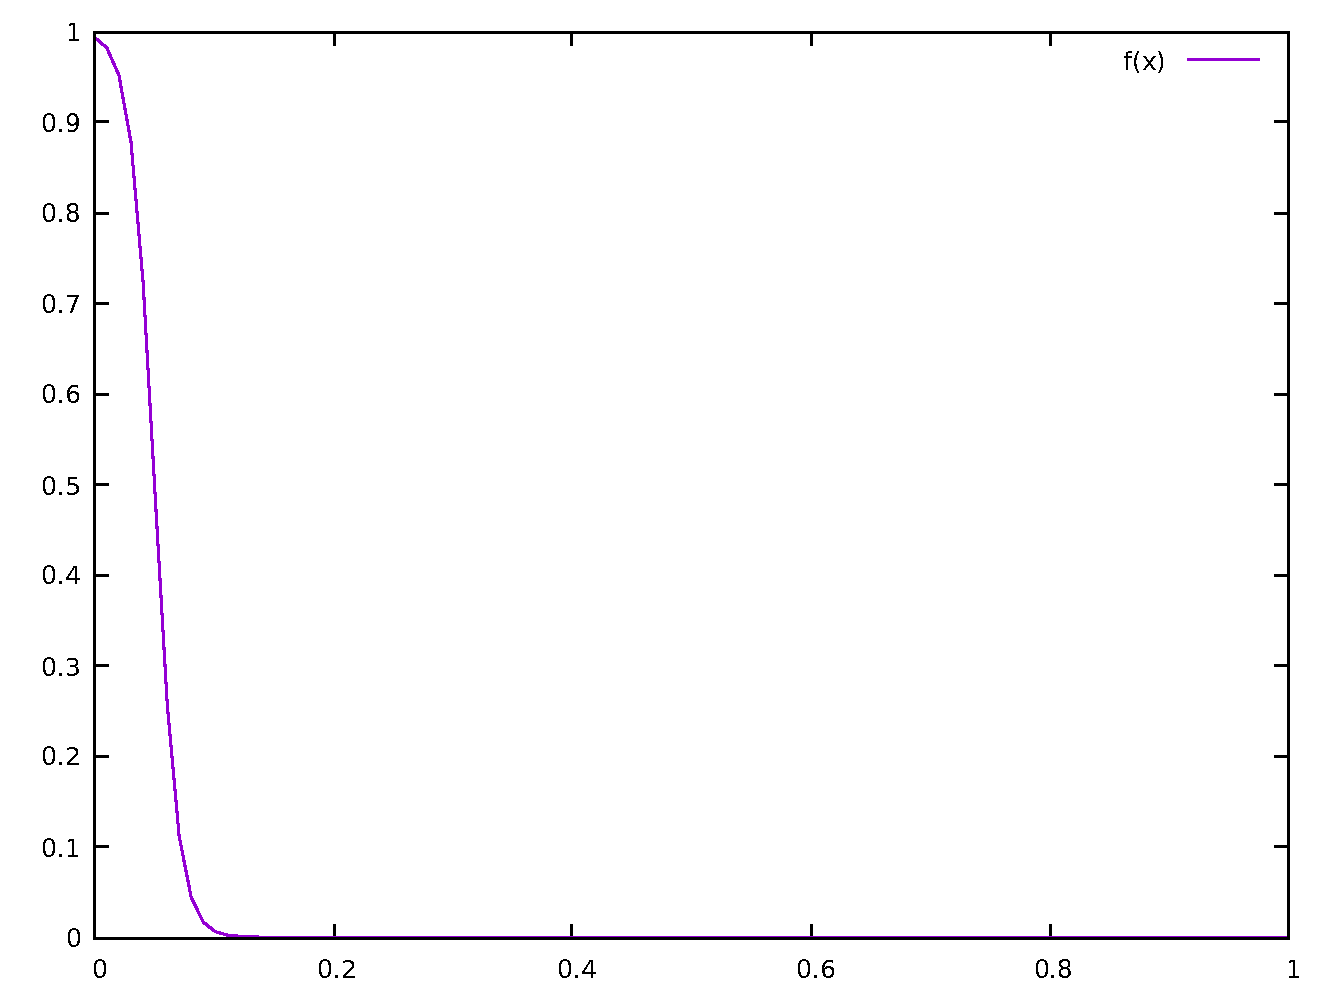
\includegraphics[height=\beamer@frametextheight]{figures/sigmoid}
        }
    }
\end{frame}
\makeatother

\begin{frame}{Petri net}

\newcommand{\nodedistance}{2}
\newcommand{\nd}[1]{\numexpr #1 * \nodedistance \relax}

\centering
\begin{tikzpicture}[node distance=\nodedistance,>=stealth',bend angle=45,auto]

  \tikzstyle{place}=[circle,thick,draw=blue!75,fill=blue!20,minimum size=6mm]
  \tikzstyle{transition}=[rectangle,thick,draw=black!75,
  			  fill=black!20,minimum size=4mm]

%  \tikzstyle{every label}=[blue!75]

  \begin{scope}
    \node [place,tokens=1] (s1) at (\nd{0}, \nd{1}) [label={[align=center]left:Receive\\ feedback}] {};
    \node [place] (s2) at (\nd{1}, \nd{2}) [label={[align=center]above:Received\\ ACK}] {};
    \node [place] (s3) at (\nd{2}, \nd{1}) [label={[align=center]right:Packets\\ in the\\ network}] {};
    \node [place] (s4) at (\nd{1}, \nd{0}) [label={[align=center]below:Open congestion\\ window (cwnd)}] {};      

    \node [transition] (e1) at (\nd{0}, \nd{0}) [label=left:Take action] {}
      edge [post] node {$a$}(s4)
      edge [pre] node {1} (s1);    
     
    \node [transition] (e2) at (\nd{2}, \nd{0}) [label={[align=center]right:Send\\ packet}] {}
      edge [pre] node {1} (s4)
      edge [post] node {1} (s3);

    \node [transition] (e3) at (\nd{2}, \nd{2}) [label={[align=center]right:Receive\\ ACK}] {}
      edge [pre] node {1} (s3)
      edge [post] node {1} (s2);

    \node [transition] (e4) at (\nd{1}, \nd{1}) [label={[align=center]left:Update\\open\\cwnd}] {}
      edge [pre] node {1} (s2)
      edge [post] node {1} (s4);
      
    \node [transition] (e5) at (\nd{0}, \nd{2}) [label={[align=center]left:Received\\ feedback}] {}
      edge [pre] node {1} (s2)
      edge [post] node {1} (s1);

  \end{scope}

\end{tikzpicture}

\end{frame}

%\begin{frame}{Preliminary results -- Experiment characteristics}
%\centering
%\begin{tabular}{rll}
%\toprule
%Parameter & Value & Distribution \\
%\midrule
%Two-way RTT when queue is 0 & $150\,$ms & constant \\
%Bottleneck bandwidth & $15\,$Mbit/s & constant \\
%Number of senders & $8$ & constant \\
%Flow length & $100\,$kB & exponential \\
%Time between flows & $0.5\,$s & exponential \\
%Simulation duration & $500\,$s & constant \\
%Buffer size & $100$ packets & constant \\
%Stochastic loss prob. & $0\%$ & constant \\
%\bottomrule
%\end{tabular}
%\end{frame}

\begin{frame}{Some data}
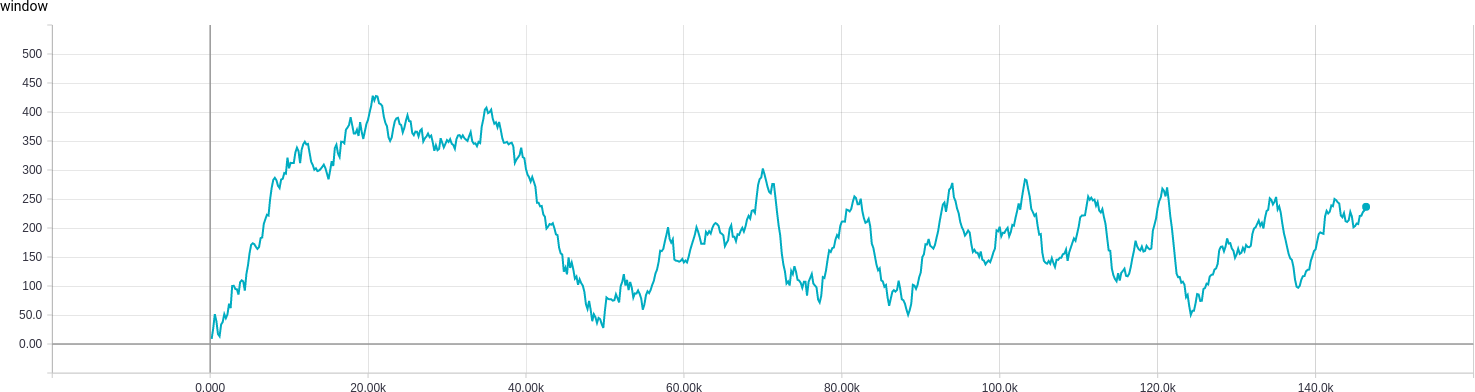
\includegraphics[width=\textwidth]{figures/window}
\end{frame}

\begin{frame}{Some data}
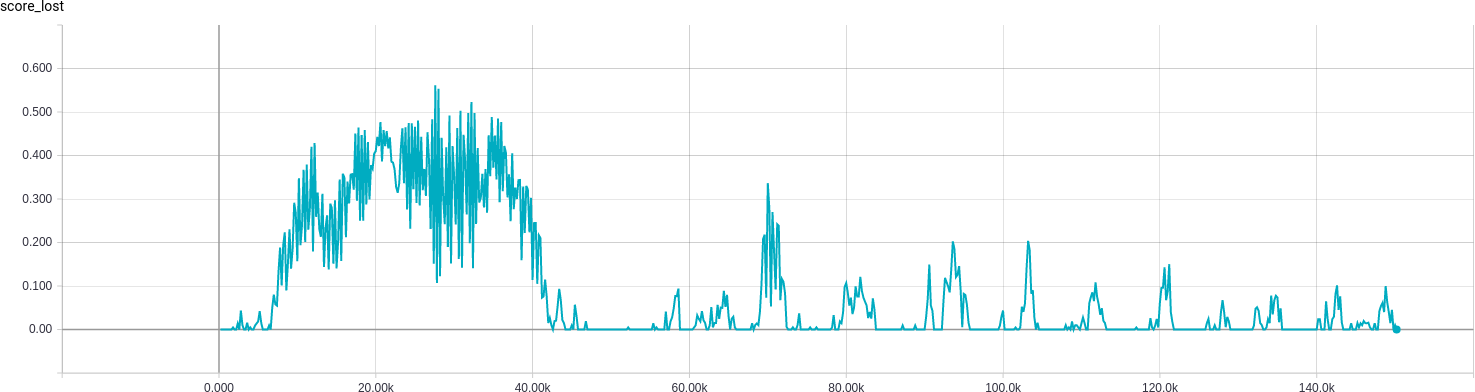
\includegraphics[width=\textwidth]{figures/score_lost}
\end{frame}

\begin{frame}{Some data}
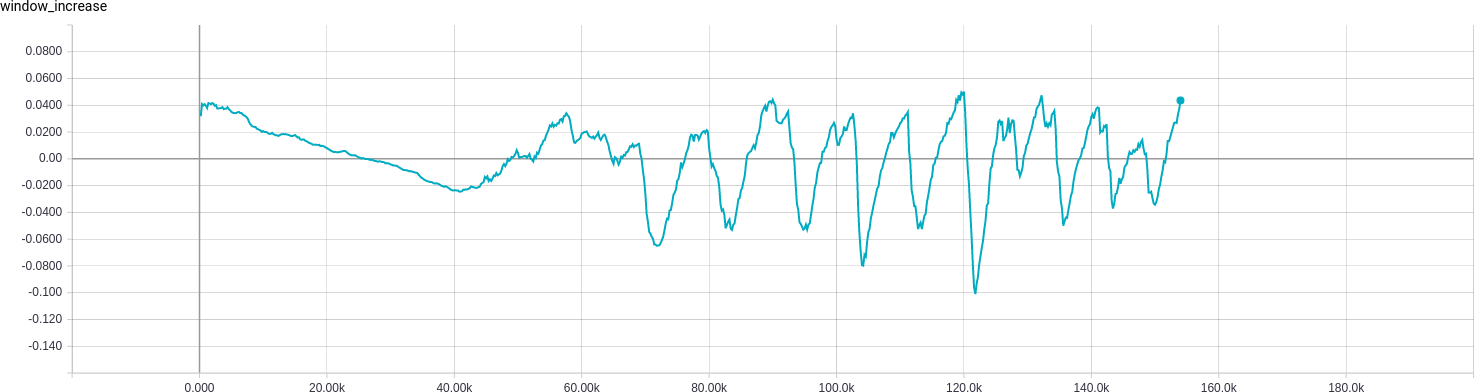
\includegraphics[width=\textwidth]{figures/window_increase}
\end{frame}

\end{document}